\documentclass[11pt]{article}

\usepackage[a4paper,margin=0.95in]{geometry}
\usepackage{amsmath,amssymb,amsthm,mathtools,bm}
\usepackage{booktabs,tabularx,array,longtable}
\usepackage{enumitem}
\usepackage{microtype}
\usepackage[hidelinks]{hyperref}
\usepackage{graphicx}
\usepackage{tikz}
\usetikzlibrary{arrows.meta,positioning,shapes.geometric,calc}

\newtheorem{assumption}{Assumption}[section]
\newtheorem{definition}[assumption]{Definition}
\newtheorem{proposition}[assumption]{Proposition}
\newtheorem{theorem}[assumption]{Theorem}
\newtheorem{lemma}[assumption]{Lemma}
\newtheorem{corollary}[assumption]{Corollary}
\theoremstyle{remark}
\newtheorem{remark}[assumption]{Remark}
\newtheorem{example}[assumption]{Example}

\newcommand{\E}{\mathbb E}
\newcommand{\Pp}{\mathbb P}
\newcommand{\R}{\mathbb R}
\newcommand{\cL}{\mathcal L}
\newcommand{\cC}{\mathcal C}
\newcommand{\cT}{\mathcal T}
\newcommand{\cH}{\mathcal H}
\newcommand{\cM}{\mathfrak M}
\newcommand{\Law}{\mathcal L}
\newcommand{\Var}{\operatorname{Var}}
\newcommand{\Cov}{\operatorname{Cov}}
\newcommand{\Corr}{\operatorname{Corr}}
\newcommand{\diag}{\operatorname{diag}}
\newcommand{\rank}{\operatorname{rank}}
\newcommand{\kernel}{\operatorname{ker}}
\newcommand{\Ran}{\operatorname{Ran}}
\newcommand{\norm}[1]{\left\lVert #1\right\rVert}
\newcommand{\abs}[1]{\left\lvert #1\right\rvert}
\newcommand{\inner}[2]{\left\langle #1,#2\right\rangle}
\newcommand{\ind}{\mathbf 1}
\newcommand{\cf}{\mathrm{cf}}
\newcommand{\obs}{\mathrm{obs}}
\newcommand{\doop}{\operatorname{do}}
\newcommand{\WT}{W_2}

\title{Work Package 8: Sharp Non-Identification Boundaries for Operator Interventions in Linear SPDEs\\
\large Feedback gauges, open-loop forcing, measurement failure, and cross-world ambiguity}
\author{}
\date{7 July 2026}

\begin{document}
\maketitle

\begin{abstract}
This note supplies the impossibility side of the operator-intervention SPDE programme. The positive theory developed in Work Packages 1--7 fixes the forcing, initial condition, noise spectrum, observation mechanism, and primitive Wiener process while replacing one operator module. We prove that these restrictions carry substantive identifying content. First, an exact decomposition gauge shows that the pairs $(A,G)$ and $(A-L,G+L\,\cdot)$ generate indistinguishable factual paths for every bounded operator $L$, although a common intervention replacing $A$ produces different post-intervention dynamics. A rank-one spectral construction gives explicit distinct Gaussian field-functional laws. Second, state feedback is not necessary for failure. We construct open-loop forcing processes that are fixed ex ante, independent of the Wiener noise, and generate either the same complete factual path or the same Gaussian law on any finite observation grid under different operators, while separating after the same operator intervention. Third, we give target-specific measurement counterexamples for rank-deficient sensing, unknown calibration, intervention-dependent measurement, and state--measurement noise decomposition. Finally, we show that identified counterfactual marginals do not identify a unit-level cross-world contrast without a coupling convention. Every result is constructive and linked to the assumption in the positive model that excludes it. Numerical calculations reproduce exact factual merging and material counterfactual separation. Work Package 8 completes the theorem architecture; only unified validation and manuscript reconstruction remain.
\end{abstract}

\section{Position and objective}

The completed theorem chain is now
\[
\mathrm{WP1}\to\mathrm{WP2}\to\mathrm{WP3}\to\mathrm{WP4}
\to\mathrm{WP5}\to\mathrm{WP6}\to\mathrm{WP7}\to\mathrm{WP8}.
\]
WP8 proves sharp impossibility results showing why the positive restrictions are needed. The remaining packages are WP9, the unified numerical and reproducibility programme, and WP10, manuscript reconstruction.

The central distinction is
\[
 \text{intervention semantics}
 \neq
 \text{identification}.
\]
A modular replacement can be mathematically well defined for each structural mechanism while its law is not determined by the factual observed distribution.

\section{Mechanisms and equivalence relations}

Let $H$ be a separable Hilbert space and let
\[
 \cM=(A,G,\Sigma,u_0,\cC,\mathcal E)
\]
denote a mechanism. Here $A$ generates a strongly continuous semigroup, $G:[0,T]\times H\to H$ is measurable and globally Lipschitz in its state argument, $\Sigma$ is a diffusion operator, $u_0$ is the initial condition, $\cC$ is an observation mechanism, and $\mathcal E$ contains measurement noise and any other declared exogenous modules. The state solves
\begin{equation}\label{eq:general}
 dU_t
 =
 \bigl(AU_t+G(t,U_t)\bigr)\,dt
 +
 \Sigma\,dW_t.
\end{equation}

\begin{definition}[Modular operator intervention]
For a declared post-intervention generator $\widetilde A$, define
\[
 I_{\widetilde A}\cM
 :=
 (\widetilde A,G,\Sigma,u_0,\cC,\mathcal E).
\]
The operator module alone is replaced.
\end{definition}

\begin{definition}[Observational and target equivalence]
For an experiment $Y$,
\[
 \cM_1\sim_{\obs}\cM_2
 \quad\Longleftrightarrow\quad
 \Law_{\cM_1}(Y)=\Law_{\cM_2}(Y).
\]
For a counterfactual target $\tau=(\widetilde A,w,z)$,
\[
 \cM_1\sim_\tau\cM_2
 \quad\Longleftrightarrow\quad
 F_\tau(\cM_1)=F_\tau(\cM_2).
\]
\end{definition}

The target is identified precisely when every observational-equivalence class is contained in a target-equivalence class. WP8 constructs explicit violations.

\begin{figure}[ht]
\centering
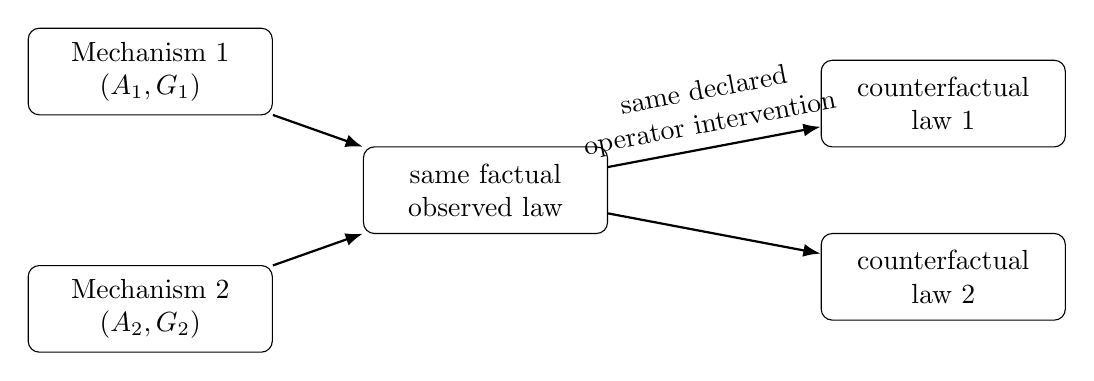
\begin{tikzpicture}[
  node distance=19mm and 27mm,
  box/.style={draw,rounded corners,align=center,minimum width=31mm,minimum height=11mm},
  arr/.style={-{Latex[length=2.2mm]},thick}
]
\node[box] (m1) {Mechanism 1\\$(A_1,G_1)$};
\node[box,below=of m1] (m2) {Mechanism 2\\$(A_2,G_2)$};
\node[box,right=of $(m1)!0.5!(m2)$] (fact) {same factual\\observed law};
\node[box,right=of fact,yshift=11mm] (cf1) {counterfactual\\law 1};
\node[box,right=of fact,yshift=-11mm] (cf2) {counterfactual\\law 2};
\draw[arr] (m1) -- (fact);
\draw[arr] (m2) -- (fact);
\draw[arr] (fact) -- node[above,sloped,align=center]{same declared\\operator intervention} (cf1);
\draw[arr] (fact) -- (cf2);
\end{tikzpicture}
\caption{Factual merging does not imply counterfactual merging.}
\label{fig:merge-split}
\end{figure}

\section{The operator--forcing decomposition gauge}

Let $A_1$ generate a $C_0$-semigroup and let $L\in\cL(H)$. Define
\begin{equation}\label{eq:gauge}
 A_2:=A_1-L,
 \qquad
 G_2(t,u):=G_1(t,u)+Lu.
\end{equation}
The bounded perturbation theorem ensures that $A_2$ is a generator with domain $D(A_2)=D(A_1)$.

\begin{definition}[Drift-decomposition gauge]
The transformation
\[
 \mathcal T_L(A,G):=(A-L,G+L\,\cdot)
\]
is called a drift-decomposition gauge transformation.
\end{definition}

\begin{theorem}[Exact factual gauge equivalence]\label{thm:gauge}
Suppose $G_1$ is globally Lipschitz. Let
\[
 \cM_1=(A_1,G_1,\Sigma,u_0,\cC,\mathcal E)
\]
and
\[
 \cM_2=(A_1-L,G_1+L\,\cdot,\Sigma,u_0,\cC,\mathcal E).
\]
Construct both equations on the same filtered probability space with the same Wiener process. Then
\[
 U_t^{\cM_1}=U_t^{\cM_2}
 \quad\text{for every }t\in[0,T]
 \quad\text{almost surely}.
\]
Consequently, every invariant observation mechanism satisfies
\[
 \cM_1\sim_{\obs}\cM_2.
\]
\end{theorem}

\begin{proof}
For $u\in D(A_1)$,
\[
 (A_1-L)u+G_1(t,u)+Lu
 =
 A_1u+G_1(t,u).
\]
Thus the two mechanisms define the same stochastic evolution equation, with the same initial condition and exogenous Wiener path. Well-posedness and pathwise uniqueness imply indistinguishability.
\end{proof}

\paragraph{Interpretation.}
Factual data can identify the total drift in \eqref{eq:general}. They cannot identify how that drift was partitioned into a module labelled ``operator'' and a module labelled ``forcing''. This is a structural equivalence, not a low-power asymptotic phenomenon.

\begin{theorem}[The intervention is not gauge invariant]\label{thm:not-descend}
Under the common intervention $I_{\widetilde A}$,
\[
 I_{\widetilde A}\cM_1
 =
 (\widetilde A,G_1,\Sigma,u_0,\cC,\mathcal E),
\]
whereas
\[
 I_{\widetilde A}\cM_2
 =
 (\widetilde A,G_1+L\,\cdot,\Sigma,u_0,\cC,\mathcal E).
\]
Their post-intervention total drifts differ by $Lu$. Therefore $I_{\widetilde A}$ does not descend to a well-defined map on the factual gauge quotient unless all admissible targets are invariant to $L$.
\end{theorem}

\begin{proof}
The displayed identities follow from modular replacement. If the intervention descended to the quotient, gauge-equivalent factual mechanisms would remain target equivalent after intervention. The rank-one construction below gives a counterexample whenever $L$ acts on a target-relevant direction.
\end{proof}

\paragraph{Assumption carrying the burden.}
The positive model fixes the forcing module. This selects one representative of the gauge class. Without that restriction, an ``operator intervention'' is representative dependent.

\section{Explicit adapted-feedback separation}

\subsection{Scalar OU model}

Let $a_0,\gamma,\sigma>0$. Consider
\begin{align}
 \cM_1:\quad
 dX_t&=-a_0X_t\,dt+\sigma\,dW_t,\label{eq:scalar1}\\
 \cM_2:\quad
 dX_t&=-(a_0+\gamma)X_t\,dt+\gamma X_t\,dt+\sigma\,dW_t.\label{eq:scalar2}
\end{align}
The factual equations are identical.

Intervene by replacing the operator rate by $\widetilde a>\gamma$. The post-intervention rates are
\[
 r_1=\widetilde a,
 \qquad
 r_2=\widetilde a-\gamma.
\]

\begin{lemma}[Integrated OU variance]\label{lem:J}
For
\[
 dX_t=-rX_t\,dt+\sigma\,dW_t,
 \qquad X_0=0,
\]
the functional $\Psi(X)=\int_0^T X_t\,dt$ is centred Gaussian with variance
\begin{equation}\label{eq:J}
 J_T(r)
 =
 \frac{\sigma^2}{r^2}
 \left[
 T-\frac{2(1-e^{-rT})}{r}
 +\frac{1-e^{-2rT}}{2r}
 \right].
\end{equation}
The map $r\mapsto J_T(r)$ is strictly decreasing on $(0,\infty)$.
\end{lemma}

\begin{proof}
Stochastic Fubini gives
\[
 \Psi(X)
 =
 \sigma\int_0^T
 \frac{1-e^{-r(T-s)}}{r}\,dW_s.
\]
It\^o isometry yields \eqref{eq:J}. For $x>0$,
\[
 \frac{1-e^{-rx}}{r}
 =
 \int_0^x e^{-ru}\,du
\]
is strictly decreasing in $r$. Squaring and integrating over $x=T-s$ proves strict monotonicity.
\end{proof}

\begin{corollary}[Scalar counterfactual separation]\label{cor:scalar}
The mechanisms \eqref{eq:scalar1}--\eqref{eq:scalar2} have identical factual path laws but
\[
 \Law\!\left(\int_0^T X_t^{(1),\doop}\,dt\right)
 \neq
 \Law\!\left(\int_0^T X_t^{(2),\doop}\,dt\right),
\]
because $J_T(\widetilde a)\neq J_T(\widetilde a-\gamma)$.
\end{corollary}

\subsection{Rank-one SPDE construction}

Let $A_0e_k=-\lambda_ke_k$ on $H$, and let $P_\ell=e_\ell\otimes e_\ell$. Set
\[
 A_1=a_0A_0,
 \qquad
 L=\gamma P_\ell,
 \qquad
 A_2=A_1-L,
 \qquad
 G_1=0,
 \qquad
 G_2(u)=Lu.
\]
The factual SPDEs coincide by Theorem~\ref{thm:gauge}.

\begin{theorem}[Field-level adapted-forcing non-identification]\label{thm:field}
Let the common intervention be $\widetilde A=\widetilde aA_0$, assume
\[
 0<\gamma<\widetilde a\lambda_\ell,
 \qquad
 q_\ell>0,
\]
and take $w_t=e_\ell$. Then the two factual field paths are indistinguishable, while the post-intervention laws of
\[
 \Psi_w(U)=\int_0^T\inner{e_\ell}{U_t}\,dt
\]
are distinct centred Gaussian laws.
\end{theorem}

\begin{proof}
The factual total generator in both mechanisms is $a_0A_0$. After intervention, mode $\ell$ has rate
\[
 r_1=\widetilde a\lambda_\ell
\]
under the first mechanism and
\[
 r_2=\widetilde a\lambda_\ell-\gamma
\]
under the second. The target uses only that mode and has variances
\[
 q_\ell^2J_T(r_1)
 \quad\text{and}\quad
 q_\ell^2J_T(r_2),
\]
with the common scale absorbed in $J_T$. Lemma~\ref{lem:J} gives strict inequality.
\end{proof}

\paragraph{Sharpness.}
The offset is harmful only when it reaches the target. If $w$ annihilates the invariant subspace on which $L$ acts and the perturbation cannot propagate into the target through the intervened dynamics, the two target laws can coincide.

\section{Open-loop exogenous forcing}

\begin{remark}[Structural rather than statistical exogeneity]\label{rem:exog}
A non-degenerate input that causes the state is generally statistically dependent on the state it produces. The relevant restriction is therefore not $F_t\perp U_t$. We call $F$ open-loop exogenous when it is generated from primitive variables before the state recursion, is not a function of the current state, and is independent of the Wiener noise and deterministic initial condition unless another dependence structure is explicitly declared.
\end{remark}

\subsection{Complete factual path equivalence}

\begin{theorem}[Full-path open-loop confounding]\label{thm:open-path}
Let $a_1\neq a_2$, let $h\in C^1([0,T])$ satisfy $h(0)=0$, and let $Z$ be non-degenerate. Define
\[
 F_i(t):=Z\bigl(h'(t)+a_ih(t)\bigr).
\]
For
\[
 dX_t^{(i)}
 =
 -a_iX_t^{(i)}\,dt+F_i(t)\,dt,
 \qquad X_0^{(i)}=0,
\]
one has
\[
 X_t^{(i)}=Zh(t)
 \quad\text{for all }t
\]
under both mechanisms. Hence their complete factual path laws coincide.

After the common intervention $a_i\mapsto\widetilde a$, holding $F_i$ fixed,
\begin{equation}\label{eq:open-cf}
 X_t^{(i),\doop}
 =
 Z\left[
 h(t)
 +(a_i-\widetilde a)
 \int_0^t e^{-\widetilde a(t-s)}h(s)\,ds
 \right].
\end{equation}
Any field functional that does not annihilate the second term has a different post-intervention law for $i=1$ and $i=2$.
\end{theorem}

\begin{proof}
Substitution gives
\[
 \frac{d}{dt}[Zh(t)]
 =
 -a_iZh(t)+Z[h'(t)+a_ih(t)].
\]
Uniqueness proves factual equality. Variation of constants under rate $\widetilde a$ yields
\[
 X_t^{(i),\doop}
 =
 Z\int_0^t e^{-\widetilde a(t-s)}
 [h'(s)+a_ih(s)]\,ds.
\]
Integration by parts gives \eqref{eq:open-cf}. The coefficient of $a_i-\widetilde a$ is non-zero for a target that sees the response direction.
\end{proof}

\paragraph{Consequence.}
State feedback is sufficient for failure but not necessary. Unknown open-loop forcing laws already destroy operator identification.

\subsection{Positive-noise finite-grid confounding}

Consider
\begin{equation}\label{eq:open-grid}
 dX_t=-aX_t\,dt+F_t\,dt+\sigma\,dW_t,
 \qquad X_0=0.
\end{equation}
Fix $0=t_0<t_1<\cdots<t_m$ and let
\[
 F_t=Z_j,\qquad t\in(t_{j-1},t_j],
 \qquad
 Z\sim N(0,K),
 \qquad
 Z\perp W.
\]
For $Y=(X_{t_1},\ldots,X_{t_m})^\top$,
\[
 Y=L_aZ+\varepsilon_a,
\]
where
\begin{equation}\label{eq:L}
 (L_a)_{j\ell}
 =
 \ind\{\ell\le j\}
 e^{-a(t_j-t_\ell)}
 \frac{1-e^{-a(t_\ell-t_{\ell-1})}}{a},
\end{equation}
and $\varepsilon_a\sim N(0,C_a^W)$. The lower-triangular matrix $L_a$ is invertible.

\begin{theorem}[Every finite Gaussian grid can be confounded]\label{thm:grid}
Fix $a_1\neq a_2$. Choose
\[
 C=MI_m,
 \qquad
 M>\max_{i=1,2}\lambda_{\max}(C_{a_i}^W),
\]
and define
\begin{equation}\label{eq:Ki}
 K_i
 =
 L_{a_i}^{-1}(C-C_{a_i}^W)L_{a_i}^{-\top}.
\end{equation}
Then $K_i$ is positive definite and both factual experiments satisfy
\[
 Y^{(i)}\sim N(0,C).
\]

Under a common intervention $a_i\mapsto\widetilde a$, the covariance is
\[
 C_i^{\doop}
 =
 C_{\widetilde a}^W
 +
 L_{\widetilde a}K_iL_{\widetilde a}^\top.
\]
For all but at most one admissible value of $M$,
\[
 C_1^{\doop}\neq C_2^{\doop}.
\]
\end{theorem}

\begin{proof}
Positive definiteness of $C-C_{a_i}^W$ and invertibility of $L_{a_i}$ imply $K_i\succ0$. Equation \eqref{eq:Ki} gives
\[
 L_{a_i}K_iL_{a_i}^\top+C_{a_i}^W=C.
\]
The counterfactual covariance difference is affine in $M$, with coefficient
\[
 L_{\widetilde a}
 \left[
 L_{a_1}^{-1}L_{a_1}^{-\top}
 -
 L_{a_2}^{-1}L_{a_2}^{-\top}
 \right]
 L_{\widetilde a}^\top.
\]
This coefficient is non-zero. Indeed, the diagonal entries
\[
 c_a(\Delta_j)=\frac{1-e^{-a\Delta_j}}{a}
\]
of $L_a$ are strictly decreasing in $a$, so $L_{a_1}L_{a_1}^\top\neq L_{a_2}L_{a_2}^\top$. An affine matrix function with non-zero slope can vanish for at most one scalar $M$.
\end{proof}

\paragraph{Interpretation.}
No finite increase in temporal resolution repairs an unrestricted-input model class. The positive experiment in WP3 is regular because the forcing law is fixed, not because the grid alone rules out latent inputs.

\begin{corollary}[One-time explicit construction]\label{cor:one-time}
At time $\Delta$, take $F_t=Z$ with $Z\sim N(0,\tau^2)$ independent of $W$. Put
\[
 c_a(\Delta)=\frac{1-e^{-a\Delta}}{a},
 \qquad
 h_a(\Delta)=\frac{1-e^{-2a\Delta}}{2a}.
\]
Then
\[
 X_\Delta\sim
 N\left(0,\tau^2c_a(\Delta)^2+\sigma^2h_a(\Delta)\right).
\]
For any
\[
 V>\max_i\sigma^2h_{a_i}(\Delta),
\]
choose
\[
 \tau_i^2
 =
 \frac{V-\sigma^2h_{a_i}(\Delta)}
 {c_{a_i}(\Delta)^2}.
\]
Both factual observations are $N(0,V)$, while after a common intervention to $\widetilde a$ their variances are
\[
 \tau_i^2c_{\widetilde a}(\Delta)^2+\sigma^2h_{\widetilde a}(\Delta),
\]
which are distinct whenever $\tau_1^2\neq\tau_2^2$.
\end{corollary}

\begin{proposition}[Unknown random initial condition]\label{prop:init}
Let $dX_t=-aX_t\,dt$ and $X_0\sim N(0,\nu_a^2)$. At a factual time $t_*$, choose
\[
 \nu_a^2=Ve^{2at_*}.
\]
Then $X_{t_*}\sim N(0,V)$ for every $a$. Under a common intervention to $\widetilde a$, holding the initial law fixed,
\[
 \Var(X_t^{\doop})=e^{-2\widetilde at}\nu_a^2,
\]
which depends on the factual representative. The deterministic-known-initial-state assumption removes this ambiguity.
\end{proposition}

\section{Measurement failures}

\subsection{Rank-deficient observation}

Let
\[
 H=H_{\obs}\oplus H_{\mathrm{lat}},
 \qquad
 \cC=P_{\obs}.
\]

\begin{theorem}[Free latent target direction]\label{thm:rank}
Suppose the model class fixes the observed block but permits the generator, noise covariance, or initial law on $H_{\mathrm{lat}}$ to vary. Then any two such mechanisms have the same complete observed factual path law. If a counterfactual target has a non-zero latent loading and the two post-intervention latent laws differ, the target is not identified.
\end{theorem}

\begin{proof}
The observation is a function only of the common observed block. Its law is therefore unchanged by latent-block modifications. A target with latent loading depends on the modified block and can separate the mechanisms.
\end{proof}

\begin{remark}[Rank deficiency is not sufficient by itself]
In the scalar positive core, known $Q$ and the common parameters $(\theta,\sigma)$ can link observed and unobserved modes. Rank deficiency becomes fatal only when $\kernel\cC$ contains a free target-relevant mechanism direction.
\end{remark}

\subsection{Unknown sensor calibration}

Consider
\[
 dX_t=-\theta X_t\,dt+\sigma\,dW_t,
 \qquad
 Y_t=cX_t.
\]
Then
\[
 dY_t=-\theta Y_t\,dt+(c\sigma)\,dW_t.
\]

\begin{proposition}[Calibration confounds field counterfactuals]\label{prop:calibration}
Let $\theta$ be common and choose
\[
 c_1\sigma_1=c_2\sigma_2,
 \qquad
 \sigma_1\neq\sigma_2.
\]
The complete factual sensor-path laws coincide. Under $\theta\mapsto\widetilde\theta$, the field law of $X^{\doop}$ depends on $\sigma_i$ and therefore differs. The sensor law of $Y^{\doop}=c_iX^{\doop}$ still depends only on $c_i\sigma_i$ and remains equal if calibration is invariant.
\end{proposition}

\paragraph{Target-specific lesson.}
Unknown calibration destroys the field-scale target but need not destroy the invariant sensor-scale target.

\subsection{Intervention-dependent measurement}

\begin{proposition}[Measurement modularity failure]\label{prop:measurement}
Suppose both factual mechanisms use the same sensor $\cC_0$, while the post-intervention sensor is unspecified and can be either $\cC_1^{\doop}$ or $\cC_2^{\doop}$. Even if $\Law(U^{\doop})$ is identified,
\[
 \Law(\cC_1^{\doop}U^{\doop})
 \neq
 \Law(\cC_2^{\doop}U^{\doop})
\]
in general. This is an under-specified joint intervention, not a failure of the field law.
\end{proposition}

\subsection{State--measurement noise decomposition}

\begin{proposition}[Noise decomposition]\label{prop:noise}
Let
\[
 Y=X+\varepsilon,
 \qquad
 X\sim N(0,q),
 \qquad
 \varepsilon\sim N(0,r),
 \qquad
 X\perp\varepsilon.
\]
The factual law identifies only $q+r$. Suppose an intervention maps $q$ to $gq$, with $g\neq1$, and leaves $r$ fixed. Two decompositions with the same $q+r$ but different $q$ have the same factual law and distinct post-intervention variances $gq+r$.
\end{proposition}

\paragraph{Scope.}
Longer time series can identify process and measurement noise under sufficient dynamic restrictions. Proposition~\ref{prop:noise} shows that the decomposition is not identified automatically.

\section{Marginal laws versus cross-world coupling}

\begin{proposition}[Counterfactual marginals do not identify unit-level effects]\label{prop:coupling}
Suppose
\[
 X^a\sim N(0,v_a),
 \qquad
 X^b\sim N(0,v_b)
\]
are identified marginal counterfactual laws. For every $\rho\in[-1,1]$, there exists a joint Gaussian coupling with
\[
 \Corr(X^a,X^b)=\rho.
\]
All such couplings preserve the marginals, while
\[
 X^a-X^b
 \sim
 N\left(
 0,
 v_a+v_b-2\rho\sqrt{v_av_b}
 \right).
\]
Thus a unit-level contrast is not identified without a cross-world coupling assumption.
\end{proposition}

\paragraph{Relation to WP1.}
The shared-Wiener construction selects a structural coupling. Independent resampling selects another. The marginal CDF, quantile, and tail results of WP4--WP7 are unaffected; only joint cross-world claims require the additional convention.

\section{Assumption-to-failure map}

\begin{longtable}{@{}p{0.27\textwidth}p{0.30\textwidth}p{0.35\textwidth}@{}}
\toprule
Positive assumption & Ambiguity removed & Failure when removed\\
\midrule
Forcing module fixed & operator/forcing decomposition & $(A,G)\sim(A-L,G+L\,\cdot)$\\
No unrestricted feedback & exact state-dependent offset & Theorems~\ref{thm:gauge}--\ref{thm:field}\\
Open-loop forcing law restricted & operator/input covariance trade-off & Theorems~\ref{thm:open-path}--\ref{thm:grid}\\
Known deterministic $u_0$ & initial-law/operator trade-off & Proposition~\ref{prop:init}\\
Target-relevant observability or cross-mode restrictions & free latent mechanism & Theorem~\ref{thm:rank}\\
Known calibration for field targets & $c\sigma$ confounding & Proposition~\ref{prop:calibration}\\
Measurement invariance & undefined observed intervention & Proposition~\ref{prop:measurement}\\
Identifiable process/measurement noise split & $q+r$ confounding & Proposition~\ref{prop:noise}\\
Shared primitive noise for unit-level effects & cross-world correlation & Proposition~\ref{prop:coupling}\\
\bottomrule
\end{longtable}

\section{Numerical validation}

The supplied script evaluates exact Gaussian laws; simulation error is not used to create the equivalences.

For the adapted-feedback example, the factual integrated-functional variance gap is numerically zero. After the common intervention, the Kolmogorov distance is approximately $0.0359$ and the Gaussian $W_2$ distance is approximately $0.0340$.

For the one-time open-loop construction, both factual variances equal $0.5$ to machine precision. The post-intervention Kolmogorov distance is approximately $0.0984$ and the $W_2$ distance is approximately $0.2910$.

For four observation times, the covariance construction gives a factual Frobenius gap of approximately $8.2\times10^{-16}$, while the post-intervention covariance gap is approximately $0.7003$.

For the calibration example, factual sensor variance and post-intervention sensor variance coincide exactly, but the field counterfactual Kolmogorov distance is approximately $0.1613$.

\begin{figure}[ht]
\centering
\includegraphics[width=.72\textwidth]{wp8_adapted_counterfactual_split.png}
\caption{Counterfactual separation after exact factual merging in the adapted-feedback construction.}
\label{fig:adapted}
\end{figure}

\begin{figure}[ht]
\centering
\includegraphics[width=.72\textwidth]{wp8_exogenous_counterfactual_split.png}
\caption{Counterfactual separation under open-loop forcing covariance confounding.}
\label{fig:exogenous}
\end{figure}

\begin{figure}[ht]
\centering
\includegraphics[width=.72\textwidth]{wp8_crossworld_coupling.png}
\caption{Different unit-level contrast laws under identical counterfactual marginals.}
\label{fig:coupling}
\end{figure}

\section{Completion and paper-facing statement}

\begin{theorem}[Sharp non-identification boundary]\label{thm:assembly}
The following enlargements of the positive model each contain two mechanisms with equal factual observed law and unequal post-intervention target law:
\begin{enumerate}[label=(\roman*)]
 \item unrestricted bounded state-feedback forcing;
 \item unrestricted open-loop forcing law, even when independent of the Wiener noise;
 \item unknown random initial law under finite observation;
 \item rank-deficient sensing with a free target-relevant latent mechanism;
 \item unknown calibration for field-scale targets;
 \item intervention-dependent measurement;
 \item non-identified state--measurement noise decomposition.
\end{enumerate}
Moreover, marginal counterfactual identification does not identify a cross-world contrast without a coupling convention.
\end{theorem}

\begin{proof}
Items (i)--(vii) are Theorems~\ref{thm:gauge}, \ref{thm:open-path}, \ref{thm:grid}, and \ref{thm:rank}, together with Propositions~\ref{prop:init}, \ref{prop:calibration}, \ref{prop:measurement}, and \ref{prop:noise}. The cross-world statement is Proposition~\ref{prop:coupling}.
\end{proof}

\paragraph{What the theorem says.}
The positive assumptions are not merely convenient regularity restrictions. They remove concrete observational symmetries that otherwise make the declared operator intervention representative dependent.

\paragraph{What remains identifiable.}
Every negative result is target specific. Sensor-scale targets can survive unknown calibration; observed-subspace targets can survive latent dynamics; marginal targets can survive cross-world ambiguity. The correct conclusion is not that causal inference for SPDEs is impossible, but that its identifying modules must be stated.

\paragraph{Programme status.}
WP8 completes the theorem system. WP9 must now consolidate all existing WP3--WP8 numerical assets into one command, add the planned high-replication heat-equation experiments, and verify every formal regime. WP10 can then reconstruct the paper around the final dependency chain.

\begin{thebibliography}{9}

\bibitem{DaPratoZabczyk2014}
G. Da Prato and J. Zabczyk.
\newblock \emph{Stochastic Equations in Infinite Dimensions}, second edition.
\newblock Cambridge University Press, 2014.

\bibitem{HannanDeistler2012}
E. J. Hannan and M. Deistler.
\newblock \emph{The Statistical Theory of Linear Systems}.
\newblock SIAM, 2012.

\bibitem{KongEtAl2022}
H. Kong, S. Sukkarieh, T. J. Arnold, T. Chen, and W. X. Zheng.
\newblock The noise covariances of linear Gaussian systems with unknown inputs are not uniquely identifiable using autocovariance least-squares.
\newblock \emph{Systems \& Control Letters}, 162:105172, 2022.

\bibitem{KongEtAl2023}
H. Kong, S. Sukkarieh, T. J. Arnold, T. Chen, B. Mu, and W. X. Zheng.
\newblock Identifiability analysis of noise covariances for LTI stochastic systems with unknown inputs.
\newblock \emph{IEEE Transactions on Automatic Control}, 68(7):4459--4466, 2023.

\bibitem{SokolHansen2014}
A. Sokol and N. R. Hansen.
\newblock Causal interpretation of stochastic differential equations.
\newblock \emph{Electronic Journal of Probability}, 19(100):1--24, 2014.

\bibitem{YongEtAl2017}
S. Z. Yong, M. Zhu, and E. Frazzoli.
\newblock Simultaneous input and state estimation for linear time-varying continuous-time stochastic systems.
\newblock \emph{IEEE Transactions on Automatic Control}, 62(5):2531--2538, 2017.

\end{thebibliography}

\end{document}
